
\documentclass[french]{article}
\usepackage{graphicx} % Required for inserting images
\usepackage{amsmath,amssymb,amsthm}
\usepackage{amsfonts}
\usepackage{babel}
\usepackage[utf8]{inputenc}
\usepackage[T1]{fontenc}
\usepackage{xcolor}
\usepackage{tikz}
\usepackage[ruled,vlined,linesnumbered]{algorithm2e}
\usepackage{algorithmic}
\newtheorem{theorem}{Définition}
\usepackage{listings}
\usepackage{xcolor}
\usepackage{seqsplit}
\usepackage{fullpage}
\usepackage{fancyvrb}
\usepackage{amsmath}
\usepackage{hyperref} \usepackage{svg}

\definecolor{codegreen}{rgb}{0,0.6,0}
\definecolor{codegray}{rgb}{0.5,0.5,0.5}
\definecolor{codepurple}{rgb}{0.58,0,0.82} \definecolor{backcolour}{rgb}{0.95,0.95,0.92}
\lstdefinestyle{mystyle}{
    backgroundcolor=\color{backcolour},   
    commentstyle=\color{codegreen},
    keywordstyle=\color{magenta},
    numberstyle=\tiny\color{codegray},
    stringstyle=\color{codepurple},
    basicstyle=\ttfamily\footnotesize,
    breakatwhitespace=false,         
    breaklines=true,                 
    captionpos=b,                    
    keepspaces=true,                 
    numbers=left,                    
    numbersep=5pt,                  
    showspaces=false,                
    showstringspaces=false,
    showtabs=false,                  
    tabsize=2
}

\lstset{style=mystyle}
\renewcommand{\qedsymbol}{$\blacksquare$}
% footnote with number
\title{Devoir 2 IFT3325}
\author{Étienne Collin,Emeric Laberge}
\date{Novembre 2023}
%\setlength{\parindent}{0pt}
\usepackage{geometry}
% \geometry{a4paper, margin=1in}
\begin{document} \title{Devoir 2 IFT3325}
\author{Étienne Collin, Emeric Laberge}
\date{\today}
\begin{titlepage}
	\begin{center}
		\vspace*{1cm}

		\Huge
		\textbf{Devoir 2}

		\vspace{0.5cm}
		\LARGE

		\vspace{1.5cm}


		\textbf{Étienne Collin}\\ 20237904 \\

		\textbf{Emeric Laberge}\\ 20220275

		\vfill

		Dans le cadre du cours\\
		IFT 3325


		\vspace{0.8cm}

		
\includegraphics[width=0.4\textwidth]{udem.jpg}

		\Large
		Département d'informatique et de recherche opérationnelle\\
		Université de Montréal\\
		Canada\\
		29 novembre 2024

	\end{center}
\end{titlepage} 

\section{Diagramme de classes} 
\begin{figure}[h]
  \centering
  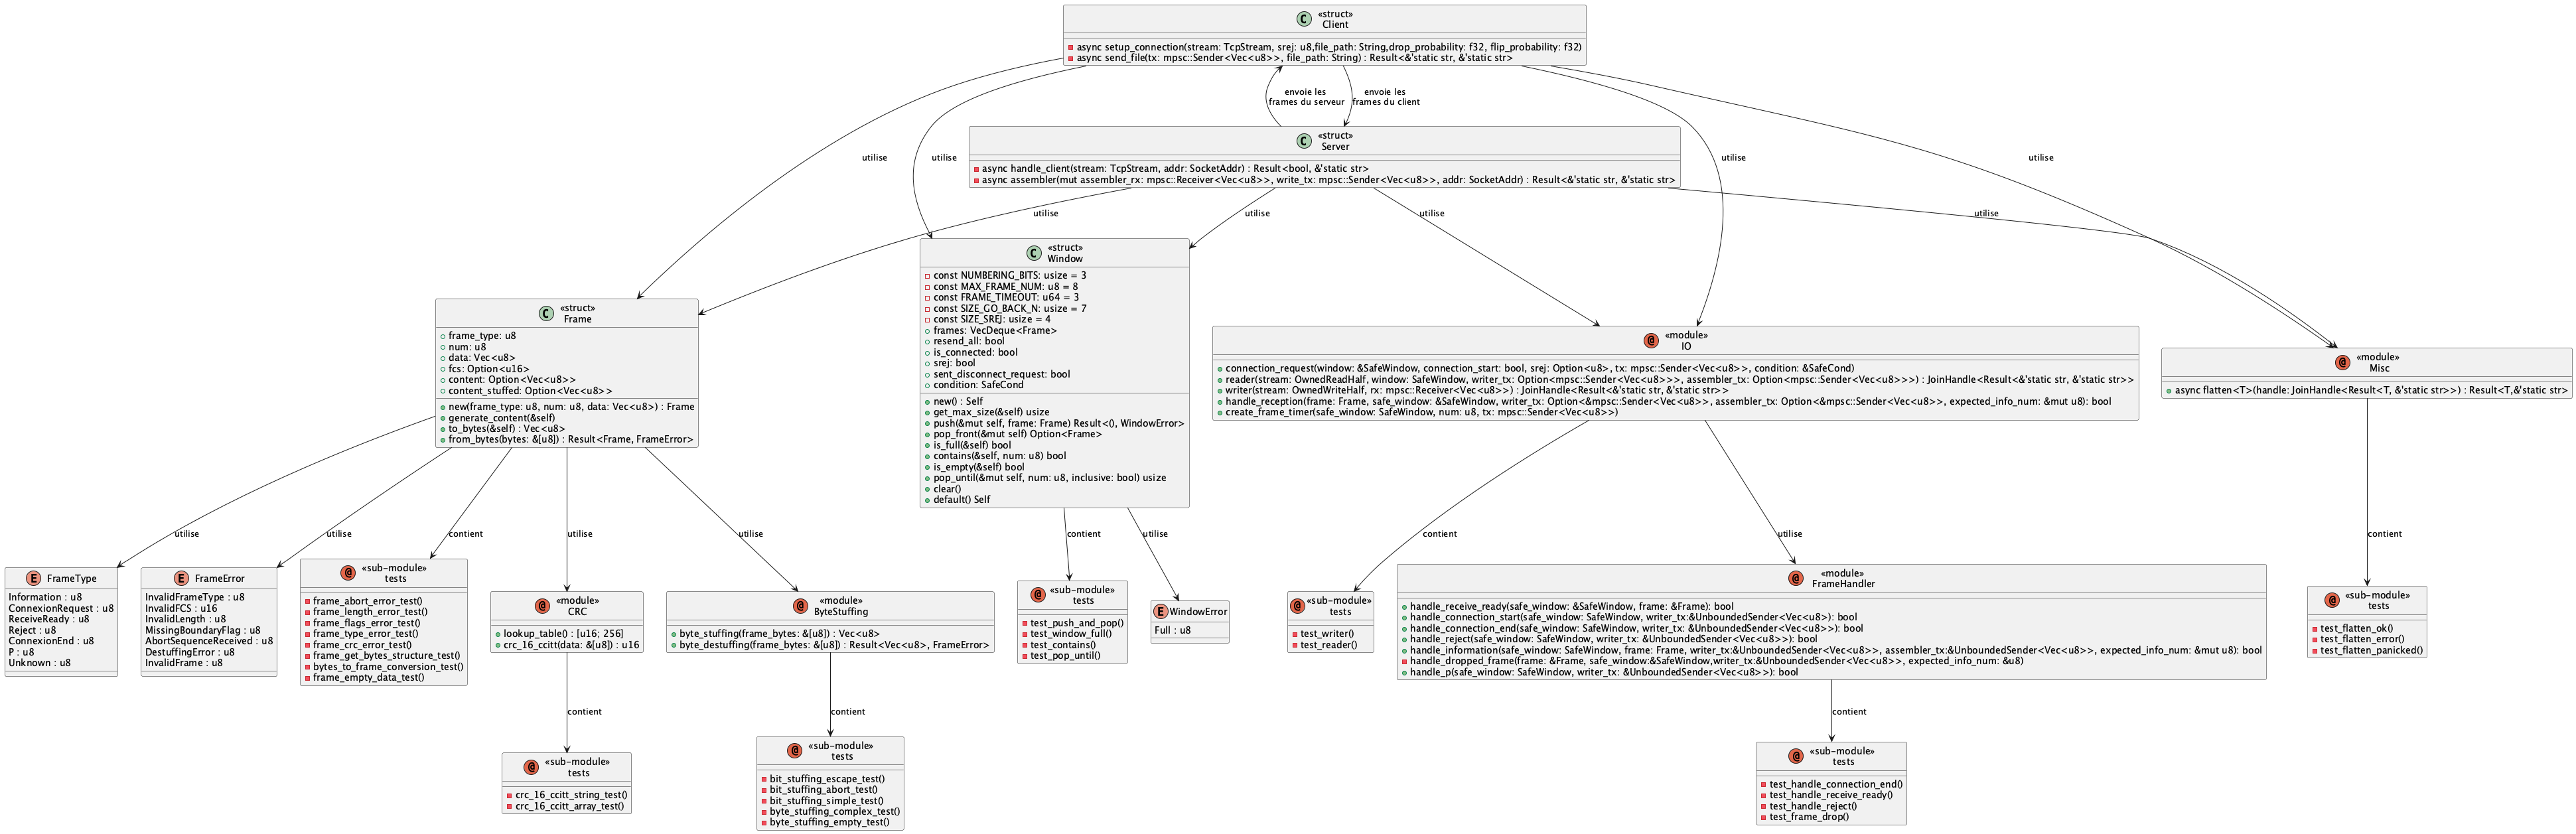
\includegraphics[width=1\textwidth]{../class-diagram/class-diagram.png}
  \caption{Diagramme de classes} 
\end{figure}

Veuillez consulter le fichier \texttt{class-diagram.svg} pour une version plus
lisible du diagramme de classes. 

\end{document}
